\begin{figure}[htbp]
\centering 
  \subfloat[Parameter space plot, $AoR_{exp} = 38.85 
        ^\circ$ \& \acs{SCT}: $\sigma_n=10070$ Pa.]{
	  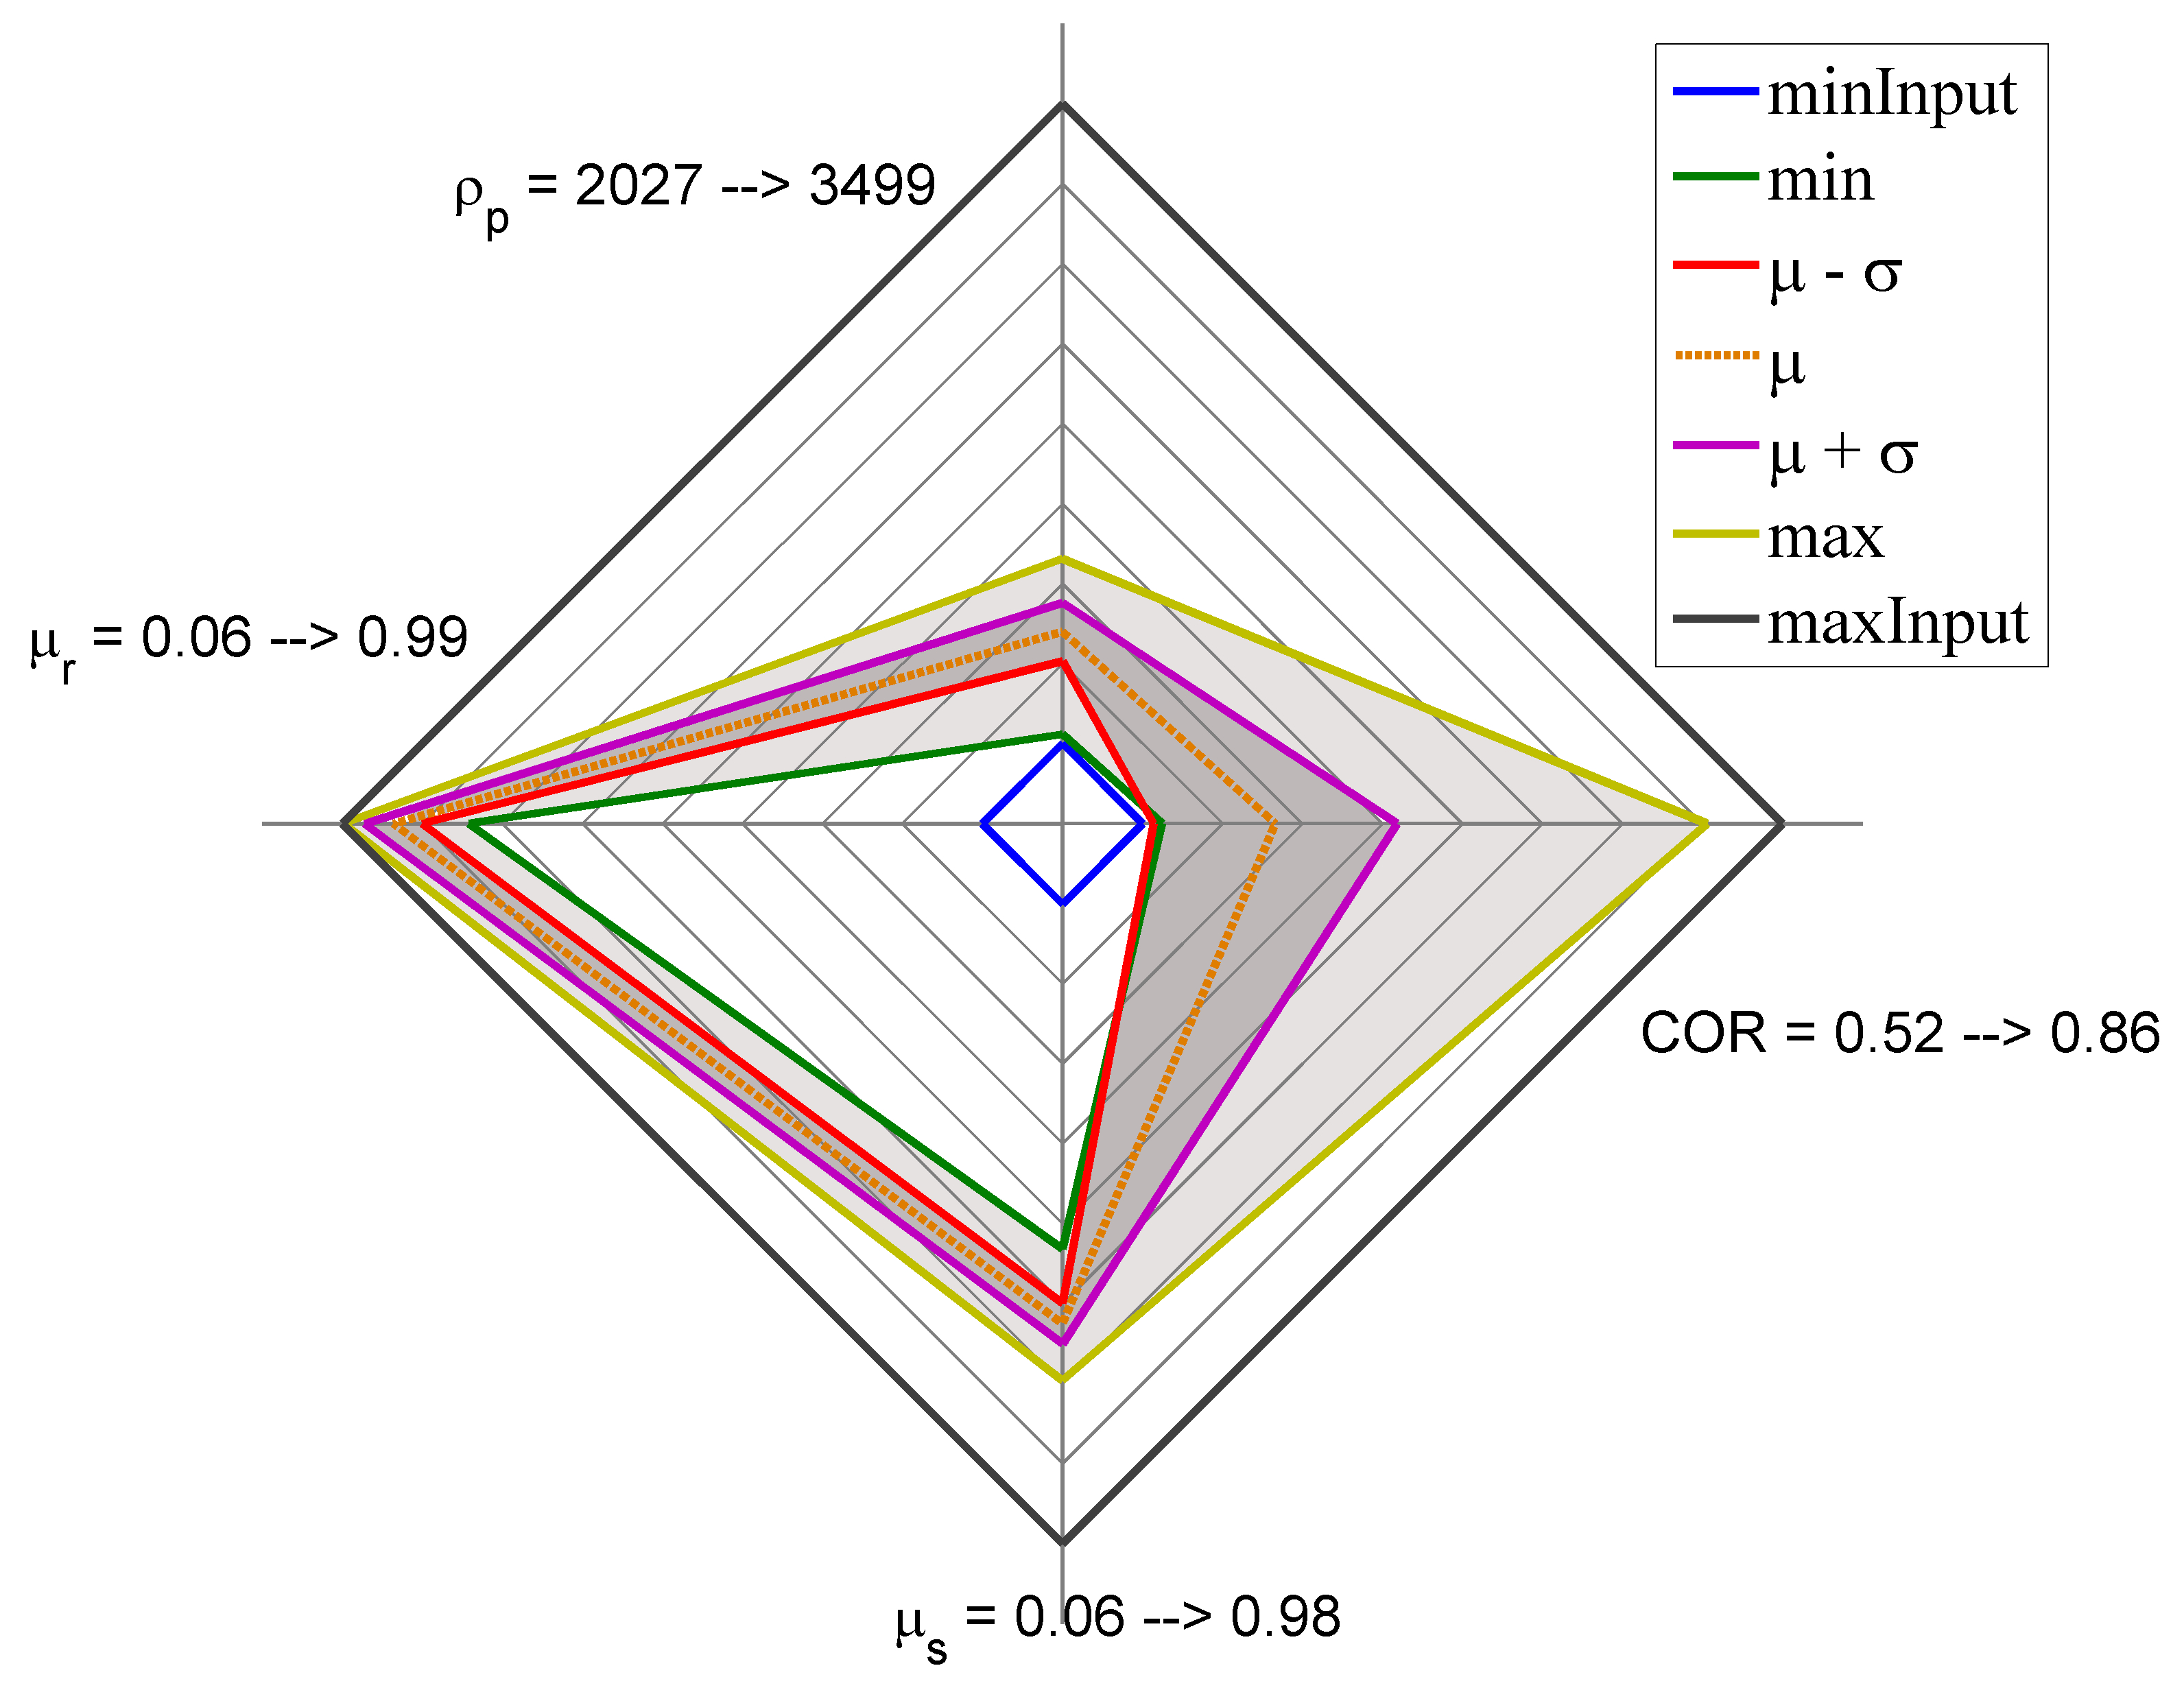
\includegraphics[width=.50\columnwidth]{images/033radarpirker1schulze10070aor}
	  \label{fig:033radarpirker1schulze10070aor}
  }
  \\
    \subfloat[Box plot, $AoR_{exp} = 38.85
        ^\circ$ \& \acs{SCT}: $\sigma_n=10070$ Pa.]{
	  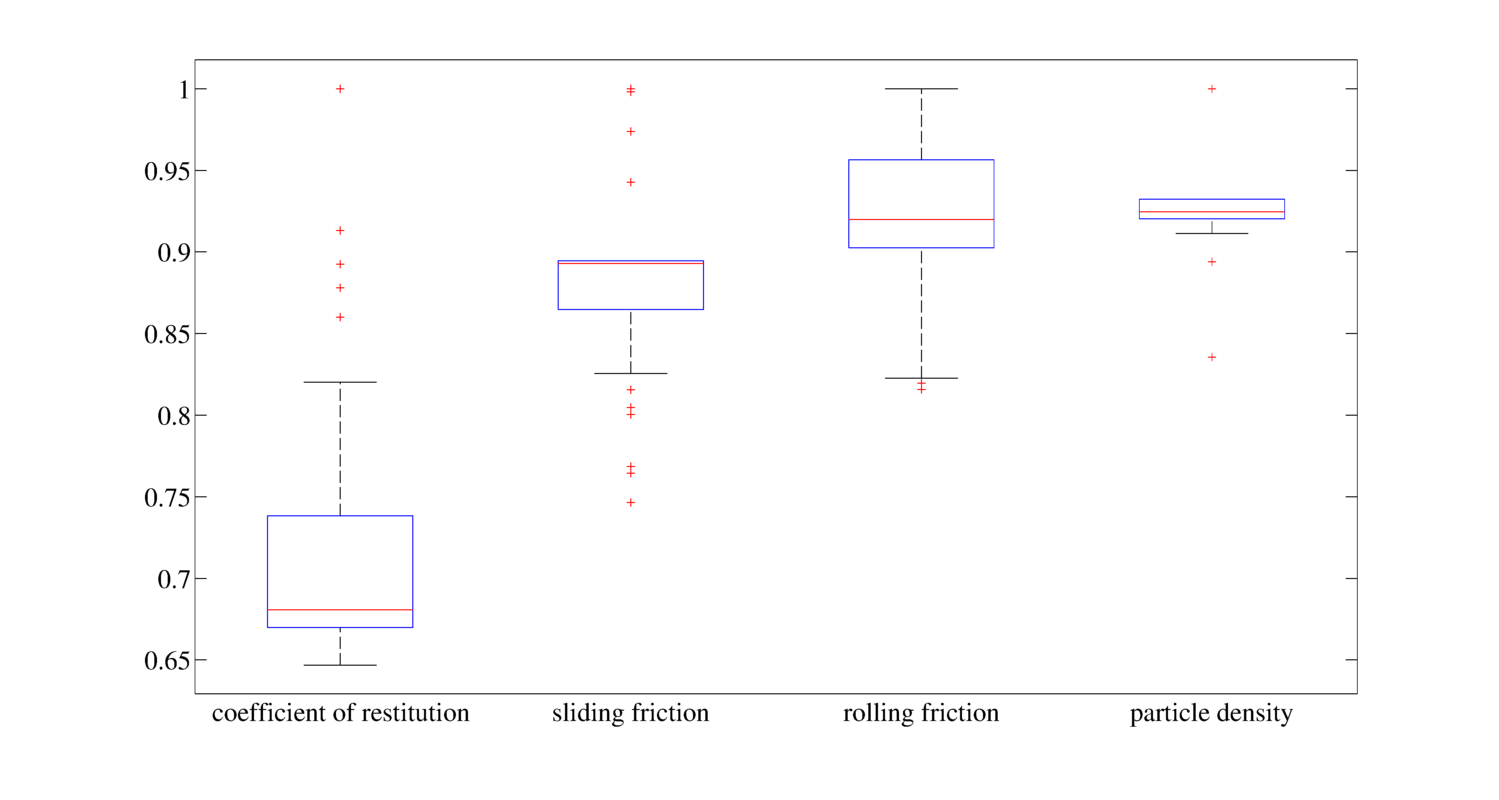
\includegraphics[width=.60\columnwidth]{images/078mergeboxplot}
	  \label{fig:078mergeboxplot}  }
  \\
  \subfloat[Density plot plot, $AoR_{exp} = 38.85 
        ^\circ$ \& \acs{SCT}: $\sigma_n=10070$ Pa.]{
	  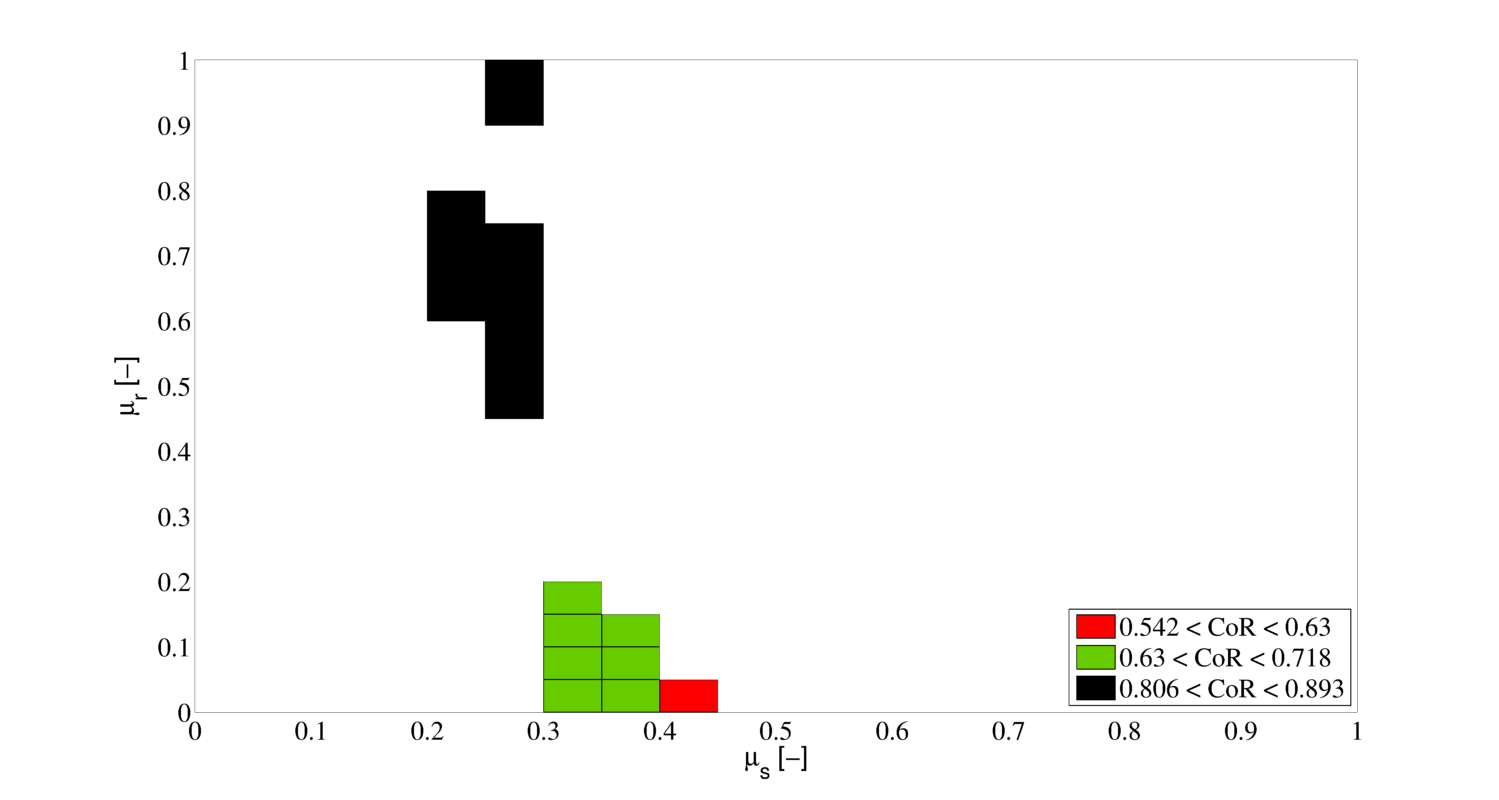
\includegraphics[width=.60\columnwidth]{images/206TileMixsinterfine_33}
	  \label{fig:206TileMixsinterfine_33}
  }
  \\  
  \caption[Merge parameter space plots of the sinter fine]{Merge parameter space
  plots of the sinter fine. A limited number of parameters are valid for both
  tests. It is clear that the friction coefficients are the most relevant micro
  parameters and only a small range of their values can be used to successfully model the bulk behaviour of the
  sinter fine.}
  \label{fig:208mergeparameterspaceplots}
\end{figure}